\chapter{Задача оптимизации направленности фазированных антенных решеток}\label{ch:ch1}

\section{Основные понятия}

Как и в работах~\cite{yurkov:groundloss,yurkov:knd} мы изучаем антенные решетки КВ диапазона, состоящие из широкополосных вертикальных
излучателей (ШВИ) см. Рис.~\ref{ris:bve_bvd}~a) и широкополосных вертикальных диполей (ШВД), см. Рис.~\ref{ris:bve_bvd}~б). Кроме того, в
рассмотрение включены решетки симметричных вертикальных диполей (СВД), см. Рис.~\ref{ris:bve_bvd}~в) и решетки ШВИ кольцевой структуры, см. Рис.~\ref{ris:bve_bvd}~г).

Каждый ШВИ состоит из 8 проводов, которые составляют ``каплеобразный'' вертикальный излучатель, обеспеченный системой противовесов.
Система противовесов каждого излучателя состоит из 6 проводов, расположенных параллельно земле. ШВД спроектирован аналогично ШВИ с той
разницей, что вместо системы противовесов подключен другой ``каплеобразный'' вертикальный излучатель, направленный в противоположную сторону. СВД являются диполями стандартной конфигурации, то есть, представляют собой прямолинейный проводник, длина которого много
больше его радиуса, питаемый от генератора посередине. Решетки ШВИ кольцевой структуры представляют собой несколько ``каплеобразных''
вертикальных излучателей, расположенных по кругу с некоторым фиксированным шагом. Система противовесов для такой решетки состоит из
радиальных проводников, причем через каждый излучатель проходит один такой проводник. Кроме того, система противовесов состоит из поперечных проводников, соединяющих соседние излучали, а также параллельных ему проводников в данном секторе. В принципе, в рассмотрение могут быть включены излучатели, спроектированные любым другим образом, если для них предоставлены соответствующие входные данные задачи оптимизации ФАР. Здесь под входными данными понимаются матрицы компонент полей и матрицы проводимости, которые можно получить с помощью некоторой программы моделирования антенн.

\begin{figure}
    \begin{minipage}[h]{0.49\linewidth}
        \center{\includegraphics[width=1\linewidth]{2x2bvm.eps} \\ а)}
    \end{minipage}
    \hfill
    \begin{minipage}[h]{0.49\linewidth}
        \center{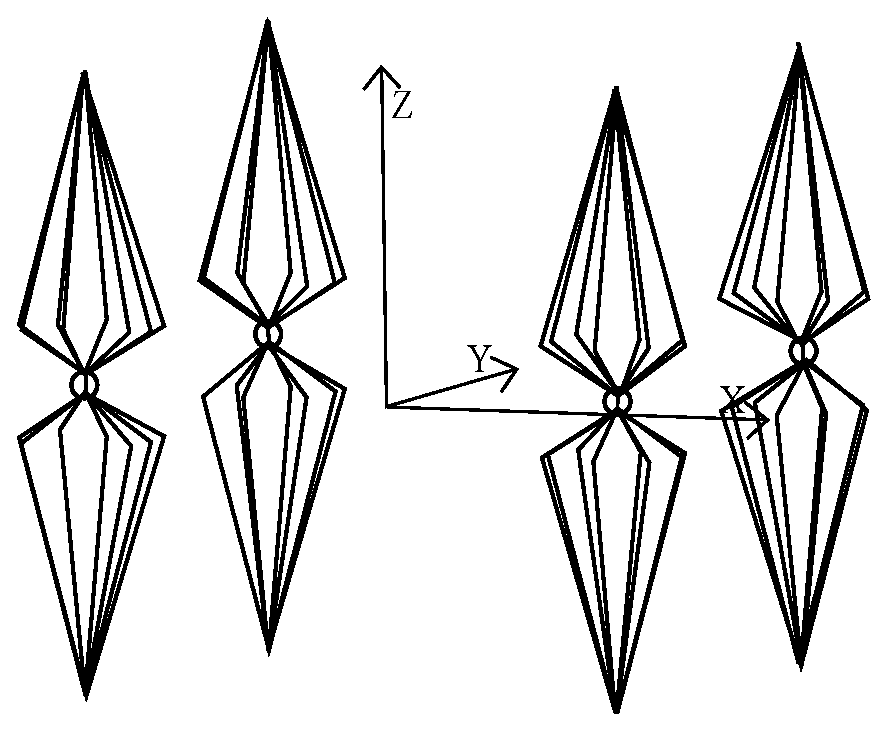
\includegraphics[width=0.6\linewidth]{2x2bvd.eps} \\ б)}
    \end{minipage}
    \begin{minipage}[h]{0.49\linewidth}
        \center{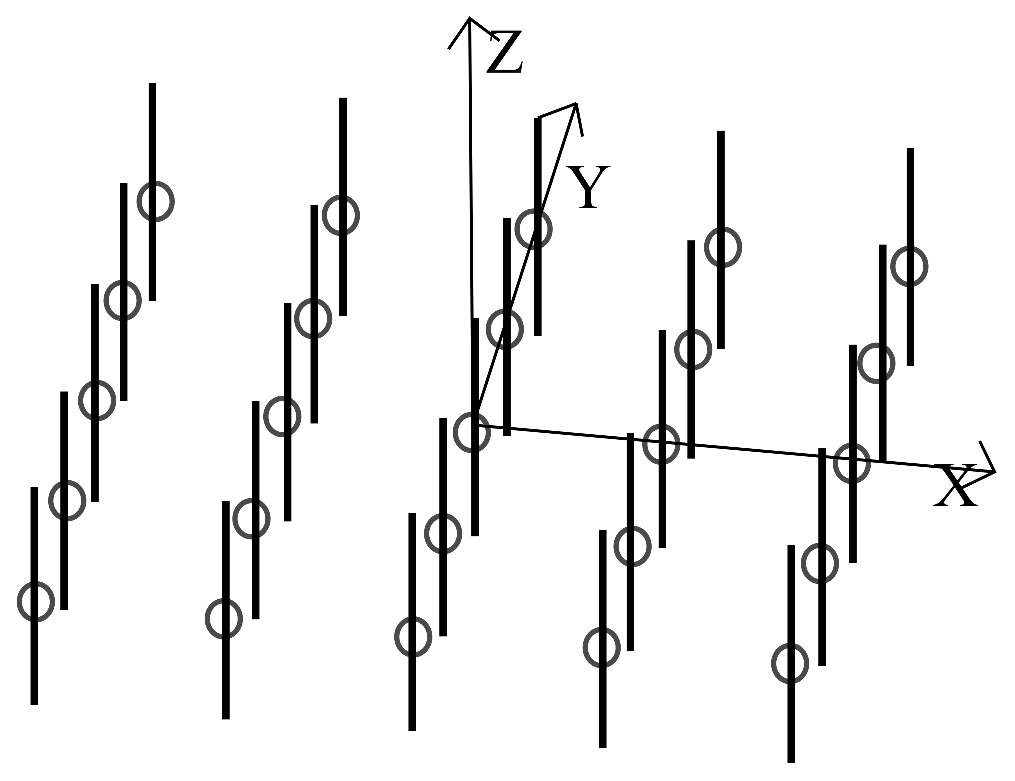
\includegraphics[width=0.6\linewidth]{5x5SVD.eps} \\ в)}
    \end{minipage}
    \hfill
    \begin{minipage}[h]{0.49\linewidth}
        \center{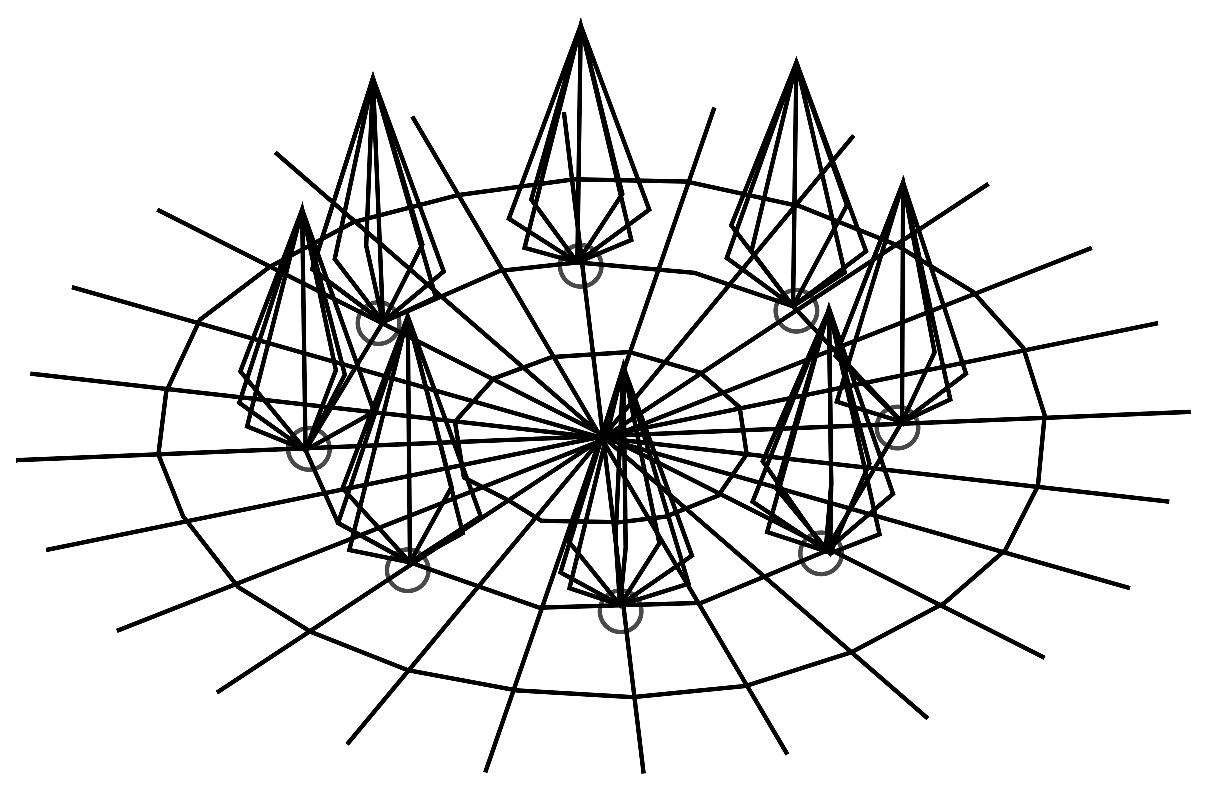
\includegraphics[width=0.9\linewidth]{r8.eps} \\ г)}
    \end{minipage}
    \caption{ФАР различных конфигураций}
    \label{ris:bve_bvd}
\end{figure}


\section{Постановка задачи}\label{sec:statement}

Нашей задачей является максимизация излучения антенной решетки в заданном направлении при ограничениях на мощность, подводимую к каждому
излучателю. В терминах комплексных токов, подводимых к излучателям, эта задача сформулирована в работах~\cite{yurkov:farkv,yurkov:knd}.
Пусть $l$ - индекс компоненты вектора направления: $l=1$ для азимутального и $l=2$ для полярного угла. Расстояние до приемника принимается во много раз превышающим размеры ФАР, поэтому индекс $l$ итерирует только эти два значения.
Суммарное электромагнитное поле $f^{(l)}_{\Sigma}$, выраженное в комплексных единицах, вводится как
%
\begin{equation}
    f^{(l)}_{\Sigma} = \sum_{i=1}^{N}I_i \tilde{f}_i^{(l)} \, ,
    \label{eq:sumfield}
\end{equation}
%
где $N$ - число точек питания антенной системы, $I_i$ - комплексный ток в $i$-й точке питания; $\tilde{f}_i^{(l)}$ - парциальное поле, то есть поле, которое излучается при подаче единичного тока на $i$-ю точку питания излучающей системы, в то время, как ток в других точках питания равен нулю. В качестве количественной меры оценки электромагнитного поля используется напряженность электрического поля. Отметим, что из определения парциального поля следует, что $\tilde{f}_i^{(l)}$ имеет размерность поля, нормированного к току. Справедливость выражения~(\ref{eq:sumfield}) следует из линейности уравнений Максвелла (более подробно см.~\cite{yurkov:farkv}). Таким образом, суммарное поле $f^{(l)}_{\Sigma}$ является суперпозицией парциальных полей от каждой точки питания излучающей системы.

Значения $f_i^{(l)}$ и $f^{(l)}_{\Sigma}$ - функции направления и частоты, которые могут быть вычислены с помощью некоторой программы моделирования антенн (здесь мы используем NEC-2~\cite{bruke:nec2}).

За $\overline{f}$ обозначим комплексное сопряжение к $f$. Как было упомянуто выше, цель - максимизация направленности излучения. В качестве количественной меры оценки направленности излучения понимается плотность мощности поля в заданном направлении, обозначаемая через $F$. Через компоненты электромагнитного поля $F$ выражается по формуле~(\ref{eq:FPrimary})
%
    \begin{equation}
        F = \sum_{l=1}^{2}\overline{f}_{\Sigma}^{(l)}f_{\Sigma}^{(l)}
        \label{eq:FPrimary}
    \end{equation}
%
и является целевой функцией задачи. При максимизации $F$ необходимо учитывать ограничения на активную мощность, которую способны выдавать усилители, питающие антенную систему. В силу закона Ома такие ограничения могут быть выражены в терминах только токов или только напряжений. Чтобы найти мощность $i$-го источника, мы вводим соответствующие комплексные напряжения~$U_i$ следующим образом:
%
    \begin{equation}
        I_i = \sum_{j=1}^{N}y_{ij}U_j \, ,
        \label{eq:om}
    \end{equation}
%
где $y_{ij}$ - элементы матрицы проводимостей $\textbf{Y} = (y_{ij})$, имеющей размерность $N \times N$.

В некоторых случаях более удобно использовать матричную нотацию. В рамках данной нотации мы вводим вектор-столбец токов $\textbf{i}$ и вектор-столбец напряжений $\textbf{u}$, состоящие из $N$ элементов. Целевая функция в таком случае формулируется следующим образом:
%
    \begin{equation}
        F = \textbf{u}^{+}\textbf{Au} \, ,
        \label{eq:F}
    \end{equation}
%
где верхний индекс $+$ означает эрмитово сопряжение, $A = (a_{ij})$,
%
     \begin{equation}
        a_{ij} = \sum_{l=1}^2\overline{f}_{i}^{(l)}f_{j}^{(l)}
        \label{eq:A} \, .
    \end{equation}
%
Соответственно, соотношение между токами и напряжениями записывается следующим образом:
%
    \begin{equation}
    \textbf{i}=\textbf{Y}\textbf{u} .
    \end{equation}
%

Существуют различные формы ограничений, которые соответствуют различным антенным системам. Например, можно ограничить суммарную мощность $P$ по всем точкам питания. В этом случае задача оптимизации формулируется так:
%
     \begin{equation}
        \begin{cases}
           \textbf{u}^{+}\textbf{Au} \rightarrow \max,\\
           \textbf{u}^{+}\textbf{Bu} = 1,
         \end{cases}
         \label{eq:task1}
    \end{equation}
%
где
%
    \begin{equation}
        \textbf{B} = \frac{1}{4P}(\textbf{Y} + \textbf{Y}^{+}).
        \label{eq:B}
    \end{equation}
%
Такая задача может быть решена аналитически~\cite{yurkov:farkv}.

Задача усложняется, когда ограничение на мощность накладывается по каждой точки питания. В этом случае задача формулируется в виде:
%
    \begin{equation}
        \begin{cases}
           \textbf{u}^{+}\textbf{Au} \rightarrow \max,\\
           0 \leq \textbf{u}^{+}\textbf{B}^{(1)}\textbf{u} \leq 1, \\
           ...\\
           0 \leq \textbf{u}^{+}\textbf{B}^{(n)}\textbf{u} \leq 1,\\
           \textbf{u} \in \mathbb{C}^N\\
         \end{cases}
         \label{eq:task2}
    \end{equation}
%
где $\mathbb{C}$ - поле комплексных чисел, $n$ - число точек питания, на которые накладываются ограничения (в общем случае $n$ может быть не равно $N$),
%
    \begin{equation}
        \textbf{B}^{(k)} = \frac{1}{4P_{max}^{(k)}}(\textbf{Y}^{+}\mathcal{P}^{(k)} + \mathcal{P}^{(k)}\textbf{Y}) \, ,
    \end{equation}
%
$P_{max}^{(k)}$ - максимально допустимая мощность в $k$-й точке питания, $\mathcal{P}^{(k)}$ - матрицы-проекторы имеющие единственный ненулевой элемент $\mathcal{P}^{(k)}_{kk}=1$. Матрицы-проекторы имеют размерность $N \times N$.

Доказано \cite{yurkov:farkv}, что:
%
\begin{enumerate}
  \item Все матрицы $\textbf{B}^{(k)}$ имеют не больше чем два ненулевых собственных значения. Одно из собственных значений положительно,
  остальные отрицательные или нулевые.
  \item Матрицы $\textbf{A}$ и $\textbf{B}^{(k)}$ эрмитово-самосопряженные, то есть
  $a_{ij} = \overline{a}_{ji}$ для всех $i = \overline{1,N}, j = \overline{1,N}$.
  \item Матрица $\textbf{A}$ положительно полуопределена.
  \item Кроме того, из физических соображений вытекает, что матрица $\textbf{B}_{\sum}:= \sum_{k=1}^{n} \textbf{B}^{(k)}$
  положительно определена, так как суммарная активная мощность, поглощаемая пассивной цепью, не может быть отрицательной либо нулем,
  поскольку, часть энергии обязательно излучится~\cite{yurkov:farkv}.
\end{enumerate}

\section{Методы решения}

В данной работе мы рассматриваем подход к решению задачи максимизации направленности излучения ФАР в заданном направлении при ограничениях, накладываемых на мощность, подаваемую на каждый из излучателей. Такая задача может быть решена только численными методами~\cite{yurkov:farkv}. Для использования градиентного метода задача сводится к задаче безусловной оптимизации методом штрафных функций. Выбор градиентного алгоритма связан с тем, что отыскание даже локального оптимума в задаче невыпуклого квадратичного программирования может представлять собой NP-трудную задачу, и одним из методов, уместных в таких случаях, является градиентный алгоритм~\cite{murty:np}. Согласно~\cite{nesterov:nonconvex}, использование метода сопряженных градиентов для решения данной задачи не будет приводить к существенным улучшениям по сравнению с простым градиентным подъемом. Данное утверждение нашло согласие с результатами предварительных вычислительных экспериментов, проведенных нами для некоторых из рассматриваемых задач.

Для оценки качества результатов градиентного алгоритма производится их сравнение с решениями, полученными с помощью решателя
BARON в пакете GAMS. BARON использует алгоритмы метода ветвей и границ, усиленные различными методами распространения ограничений и двойственности для уменьшения диапазонов переменных в ходе работы алгоритма~\cite{ryoo:nlp}. Его использование также представляет альтернативный подход к решению данной задачи, но, поскольку BARON является коммерческим решателем, произведение расчетов требует приобретения лицензии, что не всегда приемлемо.

Еще одним эффективным подоходом к решению невыпуклых задач квадратичного программирования являются генетические алгоритмы, и, в частности, методы дифференциальной эволюции (ДЭ)~\cite{storn:de,noguchi:de}. Использование методов ДЭ требует больше времени, чем использование градиентного подъема, однако, в отличие от градиентных методов, не требует вычисления производных и не подвержен преждевременному завершению в точках стационарности. Таким образом, методы ДЭ также могут быть применены при исследовании структуры локальных оптимумов задачи невыпуклого квадратичного программирования.

Вообще говоря, при использовании метода градиентного подъема не гарантируется получение глобального оптимума. Приблизиться к глобальному
оптимуму позволяет многократный запуск алгоритма из случайным образом сгенерированных точек. Кроме того, многократный запуск позволяет
оценить количество локальных оптимумов, что является некоторым критерием сложности индивидуальной задачи~\cite{eremeev:confidence}. Анализ структуры локальных оптимумов позволяет также выявить наличие нетривиальных симметрий.


\section{Формулировка задачи в действительных числах} \label{subsec:statement}

Для разработки алгоритма решения задачи удобно переформулировать ее в вещественных числах. Обозначим соответствующие матрицы: $\textbf{G} \in \mathbb{R}^{(2N)^2}$ для целевой функции и $\textbf{H}^{(k)} \in \mathbb{R}^{(2N)^2}; k = \overline{1,n}$ для ограничений. Пусть $\textbf{y} \in \mathbb{C}^N$, $\textbf{A} \in \mathbb{C}^{N^2}$, и пусть $\textbf {x} \in \mathbb{R}^{2N}$ - вектор, где первые $N$
компонент являются вещественными частями соответствующих компонент вектора~$\textbf{y}$, в то время, как остальные компоненты соответствуют мнимым, то есть:
%
    $$
    \textbf{y}_i \in \mathbb{C} \longleftrightarrow (\textbf{x}_i,
    \textbf{x}_{N+i}), \ \textbf{x}_i = Re(\textbf{y}_i), \
    \textbf{x}_{N+i} = Im(\textbf{y}_i) \, i = \overline{1,N}.
    $$
%
Через $\textbf{G} \in \mathbb{R}^{(2N)^2}$ обозначим матрицу следующего вида:
%
    \begin{equation}
        \left( \begin{array}{c | c}
            Re(\textbf{A})& -Im(\textbf{A})\\
            \hline
            Im(\textbf{A})& Re(\textbf{A})\end{array}
        \right) .
    \end{equation}
%
Легко проверить, что
    \begin{equation}
        \left(\begin{array}{c} Re(\textbf{Ay}) \\ Im(\textbf{Ay})\end{array} \right) =
        \textbf{G}\left(\begin{array}{c} Re(\textbf{y}) \\ Im(\textbf{y})\end{array}\right) .
    \end{equation}
%

Из того, что матрица $\textbf{A}$ эрмитово-самосопряженная, следует, что матрица $\textbf{G}$ симметричная. Действительно, так как матрица $\textbf{A}$ эрмитово-самосопряжена, следует симметричность $Re(\textbf{A})$ и кососимметричность $Im(\textbf{A})$. Это значит, что
%
    $$
        \textbf{G}^T = \left( \begin{array}{c | c}
            Re(\textbf{A}) & (Im(\textbf{A}))^T \\
            \hline
            (-Im \textbf{A})^T & Re(\textbf{A}) \end{array}
        \right) = \left( \begin{array}{c | c}
            Re(\textbf{A}) & -Im(\textbf{A}) \\
            \hline
            Im(\textbf{A}) & Re(\textbf{A}) \end{array}
        \right)= \textbf{G} \, .
    $$
%
Таким образом, $\textbf{G}$ является симметрической матрицей. То же самое применимо к матрицам ограничений $\textbf{H}^{(k)} \in \mathbb{R}^{(2N)^2}; k=\overline{1,n}$. В вещественных числах задача~(\ref{eq:task2}) эквивалентна следующей:
    \begin{equation}
        \begin{cases}
           \textbf{x}^{T}\textbf{Gx} \rightarrow \max,\\
           0 \leq \textbf{x}^{T}\textbf{H}^{(1)}\textbf{x} \leq 1,\\
           ...\\
           0 \leq \textbf{x}^{T}\textbf{H}^{(n)}\textbf{x} \leq 1,\\
          \textbf{x} \in \mathbb{R}^{2N}.\\
         \end{cases}
         \label{eq:task3}
    \end{equation}

Задача~(\ref{eq:task3}) имеет целевую функцию, заданную квадратичной формой с положительно полуопределенной матрицей~$\textbf{G}$. Каждое ограничение формулируется квадратичной формой, определенной симметричной матрицей~$\textbf{H}^{(k)}, k=\overline{1,n}$ с двумя парами идентичных собственных значений, два из которых положительны, а другие два отрицательны или равны нулю, все остальные собственные числа равны нулю.

Следует отметить, что задача~(\ref{eq:task2}), сформулированная в комплексных числах, имеет симметрию относительно преобразования $\textbf{u} \to e^{\emph{\textbf{j}}\phi}\textbf{u}$ всех комплексных координат (по произвольному углу~$\phi$). За $\emph{\textbf{j}}$ здесь обозначена мнимая единица. В качестве доказательства рассмотрим некоторую квадратичную форму, определенную матрицей \textbf{M}: $${(\textbf{v}e^{\emph{\textbf{j}}\phi})}^{+}\textbf{M}(\textbf{v}e^{\emph{\textbf{j}}\phi}) =
\sum_{l=1}^{N}\sum_{k=1}^{N}|v_k||v_l|m_{kl}e^{\emph{\textbf{j}}(\phi_l + \phi - \phi_k - \phi)} =$$
$$ = \sum_{l=1}^{N}\sum_{k=1}^{N}|v_k||v_l|m_{kl}e^{\emph{\textbf{j}}(\phi_l - \phi_k)} .$$

Глобально-оптимальное решение задачи невыпуклого математического программирования вида (\ref{eq:task3}) может быть найдено методом
ветвей и границ~\cite{horst:global,tawarmalani:global} или с использованием методов DC программирования~\cite{horst:handbook,strekalovsky:global}. Локально-оптимальное решение задачи может быть найдено средствами градиентной оптимизации или методом Ньютона~\cite{himmelblau:nlp}. В случае большой размерности могут быть применены различные метаэвристики(см.~\cite{eberhart:swarm,storn:de}).

%\section{Другие постановки задачи}
% TODO

\section{Верхняя оценка нормы допустимых решений} \label{subsec:top}

В вычислительных экспериментах бывает полезно ограничить множество допустимых решений задачи шаром или параллелепипедом, так как это позволяет более обоснованно выбрать начальное решение для итерационных методов с мультистартом или сократить перебор в методе ветвей и границ.

Отмеченная симметрия может найти применение для уменьшения размерности области поиска на единицу. Например, фиксируя $Im(y_{N})=0$, что эквивалентно добавлению ограничения $x_{2N}=0$ к задаче~(\ref{eq:task3}).

Кроме того, можно оценить множество допустимых решений в терминах евклидова расстояния до начала координат. Отметим, что если $\textbf{x}$ удовлетворяет всем ограничениям задачи~(\ref{eq:task3}), то
$$
\min\{\textbf{z}^T \textbf{H}_{\sum} \textbf{z} \ : \ \textbf{z}\in
\mathbb{R}^{2N}, \ ||\textbf{z}|| =1\} = \lambda_{\min},
$$
(см. например~\cite{horn:matrix}, глава~1, \S~1.0.2), мы получаем
$$
\textbf{x}^T \textbf{H}_{\sum} \textbf{x} \ge ||\textbf{x}||^2
\lambda_{\min}\ \
$$
и
\begin{equation} \label{eqn:bound}
||\textbf{x}||\le \sqrt{\frac{N}{\lambda_{\min}}}.
\end{equation}

\section{Масштабирование произвольного решения в допустимую область} \label{sec:scaling}

Для данной задачи существует преобразование, позволяющее привести к допустимой области решение $\textbf{x}$, которое нарушает только ограничивающие неравенства задачи~(\ref{eq:task3}) вида $\textbf{x}^{T}\textbf{H}^{(k)}\textbf{x} \leq 1$:

\begin{equation}
    \textbf{x}': =\alpha(\textbf{x})^{-1/2} \textbf{x} ,
    \label{eq:scale}
\end{equation}
где $\alpha(\textbf{x}):=\max_{k=\overline{1,n}} \textbf{x}^T \textbf{H}^{(k)}\textbf{x}$. Поскольку как целевая функция, так и ограничения представлены квадратичными формами, применение такой операции приведет к пропорциональному уменьшению в~$\alpha(\textbf{x})$ раз значений каждой из квадратичных форм. Другими словами, если в некоторой точке $\textbf{x}$ значения каждой из квадратичных форм, задающих ограничения, больше 0, причем значения некоторых из них больше 1, то по формуле (\ref{eq:scale}) можно определить множитель, умножение которого на вектор $\textbf{x}$ ведет к тому, что наибольшее из значений квадратичных форм, задающих ограничения, будет равно 1. Данная процедура применяется для выбора начального решения, а также для масштабирования итогового решения.

\section{Постановка вычислительного эксперимента}

Процедура решения задачи оптимизации ФАР при ограничении мощности по каждой точке питания состоит в следующем:
%
\begin{enumerate}
  \item Для каждого излучателя в решетке рассчитать парциальные компоненты полей $f_i^{(l)}, i= \overline{1,N}, l=\overline{1,2}$.
  \item Вычислить матрицы $\textbf{G}$ and $\textbf{H}^{(k)},\ k=\overline{1,n},$ из подраздела~\ref{subsec:statement}.
  \item Оценить радиус допустимой области используя формулы из подраздела~\ref{subsec:top}.
  \item Решить задачу~(\ref{eq:task3}) с дополнительными ограничениями $x_N = 0, ||\textbf{x}||\le \sqrt{\frac{N}{\lambda_{\min}}}$.
\end{enumerate}

Данный подход может гарантировать нахождение как локального, так и глобального оптимума, в зависимости от решателя, используемого на шаге~4. Как один из базовых оптимизационных методов, мы рассматриваем метод градиентной оптимизации (максимизационный вариант)
с алгоритмом одномерного поиска Дэвиса, Свенна и Кэмпи~(ДСК)~\cite{himmelblau:nlp}. Далее целевая функция задачи~(\ref{eq:task3}) будет обозначатся символом $\tilde{F}$.

В нашей работе от задачи условной оптимизации мы переходим к задаче безусловной оптимизации методом штрафных функций, а именно -
методом внешней точки~\cite{eremin:convex,aoki:mo}:
\begin{equation}
       \textbf{x}^{T}\textbf{Gx} - r\cdot \sum_{k=1}^n
       \left( \min\left(0,\textbf{x}^{T}\textbf{H}^{(k)}\textbf{x}\right) +
       \min\left(0,1-\textbf{x}^{T}\textbf{H}^{(k)}\textbf{x}\right)\right)^4 \rightarrow
       \max,
     \label{eq:task4}
\end{equation}
где $r$ - достаточно большой штрафной параметр. Глобально-оптимальное решение для задачи~(\ref{eq:task4}) может не быть допустимым для изначальной задачи~(\ref{eq:task3}), но увеличение штрафного параметра~$r$ уменьшает нарушение ограничений. Кроме того, имея решение~$\textbf{x}$, которое нарушает в задаче~(\ref{eq:task3}) только неравенства вида $\textbf{x}^{T}\textbf{H}^{(k)}\textbf{x} \leq 1$, мы будем ссылаться на результаты градиентной оптимизации с использованием восстановления допустимости~(\ref{eq:scale}) после срабатывания критерия остановки. Алгоритм градиентной оптимизации повторяется многократно, при этом используется случайно сгенерированный вектор~$\textbf{x}\in \mathbb{R}^{2N}$ в качестве стартовой точки. Распределение случайной величины $\textbf{x}$ описано в подразделе~\ref{subsec:results}. Для каждого найденного решения выполняется проверка на удовлетворение необходимым условиям локальной оптимальности путем решения задачи~(\ref{eq:task5}). Затем, решение линеаризованной задачи, удовлетворяющее  необходимым условиям локальной оптимальности, снова подается на вход алгоритма градиентной оптимизации, остальные решения отсеиваются. Последний шаг применяется, поскольку решение задачи~(\ref{eq:task5}) может оказаться за пределами допустимой области задачи~(\ref{eq:task3}). В этом случае данный этап показывает, как далеко решение линеаризованной задачи находится от решения, найденного градиентным алгоритмом.

С целью отыскания глобального оптимума задачи~(\ref{eq:task3}) посредством решателя BARON~\cite{tawarmalani:global}, основанного на методе ветвей и границ с использованием локальной оптимизации для поиска начального приближения, необходимо предоставить ограничивающий параллелепипед или верхнюю оценку евклидовой нормы допустимых решений. Для этого может быть использовано неравенство~(\ref{eqn:bound}). Для всех решаемых в этом эксперименте задач была рассмотрена возможность применения процедуры сужения допустимой области.

\subsection{Тестовые примеры}\label{subsec:examples}

Вычислительный эксперимент был поставлен для задач, построенных на основе четырех типов ФАР: широкополосных вертикальных излучателей, широкополосных вертикальных диполей и симметричных вертикальных диполей. При моделировании полей был использован пакет NEC2, для которого были предоставлены соответствующие геометрические конфигурации антенных систем. В качестве рабочей частоты было выбрано 5МГц. Рассмотрены квадратные ФАР конфигурации 2x2, 3x3 и 5x5. Заранее отметим, что конфигурация 5x5 была рассмотрена только для решеток СВД, поскольку NEC2 не смог обработать 5x5~ШВИ и 5x5~ШВД из-за высокой сложности этих моделей. В случае с ФАР кольцевой структуры были рассмотрены решетки, состоящие из 8 и 16 излучателей.

Решетки ШВИ смоделированы расположенными на высоте 0.2 метра над поверхностью земли (проводимость земли равна~0.01~См/м, относительная диэлектрическая проницаемость~10). Решетки ШВИ и СВД размещены в свободном пространстве. В случае ШВЕ и ШВД, расстояние между соседними излучателями равно 20~метров. Высота каждого излучателя ШВИ равна 15~метров. Расстояния между концами каждого излучателя ШВД равно 30 метров. В случае СВД, были рассмотрены два типа излучателя: с длинами излучателя~10~и~30~метров и расстояниями между соседними излучателями 5 и 10 метров соответственно. СВД с длиной излучателя равной 10~метрам в исследовании помечены штрихом (СВД'). Система противовесов ФАР кольцевой структуры поднята над землей на 2 м. для того, чтобы ослабить влияние потерь в земле. Расстояние между соседними излучателями в этих ФАР равно 8 м. В качестве направления максимизации излучения выбраны: азимутальный угол $45^{\circ}$, полярный угол $70^{\circ}$.

\subsection{Результаты вычислительного эксперимента} \label{subsec:results}

В этом разделе мы сравниваем результаты работы градиентного метода и решателя BARON в его режиме по умолчанию. Во всех экспериментах, описанных ниже, было установлено ограничение по времени 1000с. Все эксперименты проводились на ЭВМ с процессором Intel i7 (тактовая частота: 2.8ГГц), ОЗУ: 16Гб. В случае сходимости градиентного метода (завершение по минимально допустимому приращению целевой функции $10^{-4}$), алгоритм перезапускается заново до истечения запаса времени.

Для каждой задачи была применена процедура получения верхней оценки нормы допустимых решений~(c.м. подраздел \ref{subsec:top}). При выполнении этой процедуры для многих задач получались близкие к нулю (или даже нулевые) собственные числа, что делало невозможным их дальнейшее использование для оценки нормы $\sqrt{\frac{N}{\lambda_{\min}}}$. В таблице~\ref{tab:results} такие оценки задачи отмечены прочерком в соответствующем столбце. Так как из физических соображений собственные числа должны быть строго больше 0, проблемы с вычислением верхней оценки нормы допустимых решений свидетельствуют о допущенной погрешности при вычислении матриц, определяющих квадратичные формы задачи~(\ref{eq:task3}). В частности, одной из таких проблем является несимметричный вид вещественных матриц. В таком случае, их следует привести к симметричному ввиду путем усреднения симметричных относительно главной диагонали компонент.

Во время каждой инициализации градиентного метода стартовая точка~$\textbf{x}$ выбирается независимо с равномерным распределением в кубе $[-5000, 5000]^{2N}$. Такой выбор оказался достаточным для всех задач, кроме СВД~2x2, чтобы получить решение, по целевой функции соответствующее решению, предоставляемому решателем BARON. Лучшее из найденных таким образом решений принимается за конечный результат. Параметр штрафа~$r$ в методе градиентной оптимизации установлен равным $10^6$ на всех запусках. Такое значение было определено эмпирически. В таблице~\ref{tab:results} приводятся результаты вычислительного эксперимента. Значения целевой функции ``$\tilde{F}$'' точке, полученной алгоритмом градиентного подъема, приводятся после процедуры масштабирования~(\ref{eq:scale}). Для решателя BARON версии~18.5.8 было выбрано то же самое ограничение сверху на процессорное время, что и для градиентного метода (группа колонок ``BARON''), и 50000с. для проверки глобальной оптимальности. Во всех таблицах, колонка ``t'' содержит время до получения лучшего найденного решения или до установления глобальной оптимальности. Во всех запусках градиентного метода были получены решения, где активными оказались все ограничения вида $\textbf{x}^{T}\textbf{H}^{(k)}\textbf{x} \leq 1$.

\begin{table}[!h]
\centering
\caption{ Результаты оптимизации, полученные с помощью градиентного подъема и коммерческих решателей}
\begin{tabular}{|c|c|c c|c c|}
    \hline
    \multirow{2}{*}{\textbf{Тип}} & \multirow{2}{*}{$\sqrt{\frac{N}{\lambda_{\min}}}$} & \multicolumn{2}{c}{\textbf{Град.}} & \multicolumn{2}{|c|}{\textbf{BARON}}\\
    & & \textbf{$\tilde{F}$} & \textbf{t, c} & \textbf{$\tilde{F}$} & \textbf{t, c} \\
    \hline
    ШВИ 2х2 & 13.6 & 138.2 & \textbf{0.054} & \textbf{139.2} & 0.12 \\
    ШВИ 3х3 & 22.5 & 575.7 & 0.93 & \textbf{580.6} & \textbf{0.34} \\
    ШВД 2х2 & 21 & 459.7 & \textbf{0.13} & \textbf{463.6} & 0.27 \\
    ШВД 3х3 & 82.2 & 915 & 24.4 & \textbf{925} & \textbf{0.34}  \\
    СВД 2х2 & 44.7& 357 & 1.9 & \textbf{361} & \textbf{0.16} \\
    СВД 3х3 & 641.9& 1138 & 25.6 & \textbf{1261} & \textbf{0.38}\\
    СВД 5х5 & $1.1\cdot10^{5}$ & 5318 & 1000 & \textbf{6716} & 1000 \\
    СВД' 2х2 & $2.3\cdot10^{4}$ & 233 & 2.52 & \textbf{253} & \textbf{0.25} \\
    СВД' 3х3 & $6\cdot10^5$& 664 & 71 & \textbf{1153} & \textbf{1.48} \\
    СВД' 5х5 & - & \textbf{1382.7} & 1000 & 33.5 & \textbf{217.94}  \\
    Кольц. 8 & 87 & 217 & 8.06 & \textbf{218} & \textbf{0.23} \\
    Кольц. 16 & 154 & 727 & 90.9 & \textbf{734} & \textbf{1.37} \\
    \hline
\end{tabular}
\label{tab:results}
\end{table}

Из таблицы~\ref{tab:results} видно, что на всех видах решеток, кроме решеток СВД конфигураций~3x3 и~5x5, а также СВД' конфигураций~2x2 и~3x3, разница в значениях целевой функции не превосходит 1\%. Для решеток СВД конфигураций~3x3 и~5x5, а также СВД' конфигураций~2x2 и~3x3 градиентный алгоритм существенно уступает по качеству найденного решения. Более детальное исследование для СВД' конфигураций 2x2 и 3x3 показало, что BARON предоставляет решение с очень малой областью притяжения. Суть такого исследования заключалась в том, что к решению, полученному с помощью решателя BARON добавлялось некоторое возмущение, после чего модифицированная точка подавалась на вход градиентного алгоритма. Очень малые возмущения (до 0.5\% относительно нормы решения) исходной точки не мешали градиентному алгоритму найти точку, лежащую в окрестности решения, найденного с помощью решателя BARON. Однако, принимая на вход возмущенное порядка 0.5\% относительно нормы решение решателя BARON, градиентный подъем приводил к решению со значением целевой функции $\tilde{F} = 233$  в случае СВД'~2x2. При этом, используемая нами процедура проверки локальной оптимальности не дала опровержения локальной оптимальности решения со значением целевой функции $\tilde{F} = 253$, предоставленного решателем BARON. Аналогичные результаты были получены как для СВД, так и для СВД' конфигурации~3x3. Особое внимание привлекают решетки СВД и СВД' конфигурации 5x5, поскольку за предоставленный временной промежуток градиентный подъем так и не достиг критерия остановки. BARON в случае СВД'~5x5 за это же время достиг решения, значительно хуже по целевой функции. Вероятно, как BARON, так и градиентный подъем сошлись бы к более качественному решению, если бы не были ограничены по времени. Кроме решeток ШВИ и ШВД конфигурации~2x2 BARON демонстрирует лучшее время счета. Однако, следует отметить, что для обоих алгоритмов время, затраченное на поиск решения, было либо существенно меньше, либо сравнимо со временем, затраченным на построение исходных данных пакетом моделирования NEC, что делает оба подхода равноценными по времени работы с практической точки зрения. Важным результатом, не приведенным в таблице~\ref{tab:results}, является то, что для ФАР конфигураций ШВИ~2x2, ШВД~2x2 и ШВИ~3x3 была доказана глобальная оптимальность найденного решателем BARON решения.

В качестве иллюстрации физических свойств полученных решений, на рис.~\ref{ris:bve_comp} приведен горизонтальный план диаграммы направленности ФАР для решений, найденных с помощью метода градиентной оптимизации. Под диаграммой направленности понимается графическое представление зависимости коэффициента усиления антенны от ее направления в заданной плоскости. Такая диаграмма позволяет наглядно оценить, на какое направление приходится максимум излучения, и провести качественную оценку работы алгоритма. На рис.~\ref{ris:bve_comp} изображена диаграмма направленности для решетки ШВИ размера 2x2 (пунктирная линия) и ШВИ 3x3 (сплошная линия). Для решений, полученных с помощью решателя BARON для этих задач, диаграммы аналогичны. Еще раз отметим, что при эксперименте направление оптимизации было представлено углами в полярных координатах: азимутальный угол был принят равным $45^{\circ}$, полярный угол - $70^{\circ}$. Как видно из горизонтального плана диаграммы направленности при значении полярного угла $70^{\circ}$, максимальному излучению соответствует направление оптимизации $45^{\circ}$. Сравнение диаграмм показывает, что использование решеток с большим числом излучателей позволяет уменьшить излучение в других направлениях.

\begin{figure}[h]
    \centering
    \center{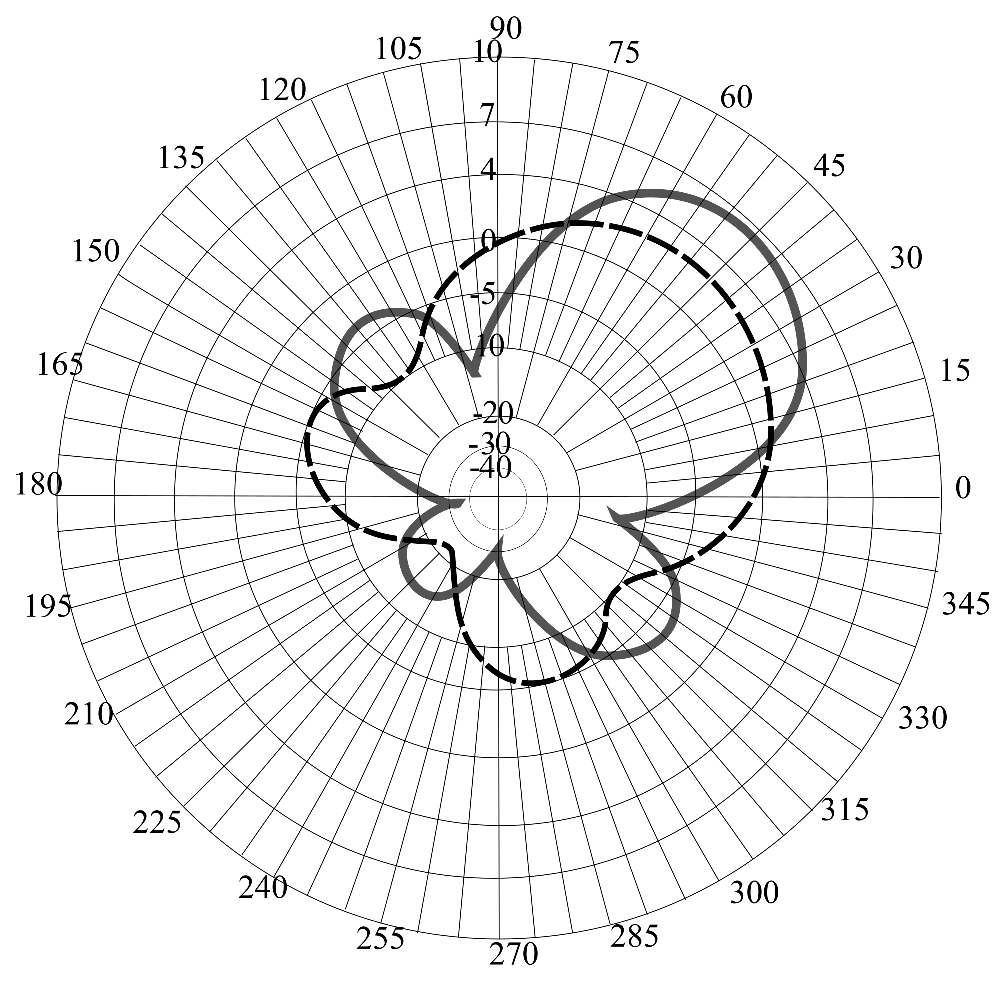
\includegraphics[width=0.5\linewidth]{BWE_comp.eps} }
    \vspace{0.7em}
    \caption{Горизонтальный план диаграммы направленности для решетки ШВИ 2x2 (пунктир) и ШВИ 3x3 (сплошная)}
    \label{ris:bve_comp}
\end{figure}
Результаты данного раздела были представлены в~\cite{tyu:daor,tyu:opta,tyu:fmh}. 